%\documentclass[notes]{beamer}       % print frame + notes
%\documentclass[notes=only]{beamer}   % only notes
\documentclass{beamer}              % only frames
%\usetheme{Darmstadt}
\usepackage{mystyle}
%\usepackage{pdfpcnotes}
\usepackage{multimedia}
%\input{math_commands.tex}
\usepackage{media9}


\title{Advanced Doctoral Studies}
\author{Abdalaziz Rashid}
\institute[HSE]{Higher School of Economics (HSE)}
\date{\today}


\begin{document}
\frame{\titlepage}


%%%%%%%%%%%%%%%%%%%%%%%%%%%%%%%%%%%%%%

\begin{frame}
\frametitle{Education}
\begin{itemize}
 \item<1-> Bachelor's Degree in Petroleum Engineering
 \item<2-> Master's Degree with Honors in Computer Science and Engineering 
\end{itemize}
\end{frame}

%%%%%%%%%%%%%%%%%%%%%%%%%%%%%%%%%%%%%%

\begin{frame}
\frametitle{Summer Schools}
\begin{itemize}
 \item<1-> New Technologies to Search for New phenomena in Particle Physics (MISIS)
 \item<2-> Six\textsuperscript{th} Machine Learning in High Energy Physics Summer School (EPFL)
 \item<3-> Summer School of Machine Learning (Skoltech)
\end{itemize}
\end{frame}

%%%%%%%%%%%%%%%%%%%%%%%%%%%%%%%%%%%%%%

\begin{frame}
  \frametitle{Career}

\begin{itemize}
  \item<1-> Data Scientist at ITCanFly (Moscow)
  \item<2-> Data Scientist at Wonderobe (Moscow)
  \item<3-> Research Assistant at Laboratory of Methods for Big Data Analysis (HSE)
\end{itemize}
\end{frame}

%%%%%%%%%%%%%%%%%%%%%%%%%%%%%%%%%%%%%%

\begin{frame}
\frametitle{Research}
      \textbf{A New Approach for Analyzing Auger Electron Spectroscopy Data Using Deep Learning}
      \begin{figure}
        \includegraphics[height=6cm, keepaspectratio]{phi680.jpg}
      \end{figure}
\end{frame}

%%%%%%%%%%%%%%%%%%%%%%%%%%%%%%%%%%%%%%

\begin{frame}
\frametitle{Research}
  \textbf{Input Data}
      \begin{figure}
        \includegraphics[width=1\textwidth]{specs.png}
      \end{figure}
\end{frame}

%%%%%%%%%%%%%%%%%%%%%%%%%%%%%%%%%%%%%%

\begin{frame}
\frametitle{Research}
  \textbf{Elemenents Identifcation and Quantification}
      \begin{figure}
        \includegraphics[width=\textwidth,keepaspectratio]{auger_peaks.png}
      \end{figure}
\end{frame}


%%%%%%%%%%%%%%%%%%%%%%%%%%%%%%%%%%%%%%

\begin{frame}
\frametitle{Research}
      \textbf{Inverse Simulation}
      \begin{itemize}
        \item<1-> Simulation 

          Solve a forward problem how a given system would behave when given a
          certain input

        \item<2-> Inverse Simulation

          Given the observed data and a simulator, infer the system parameters
          that would make the simulator data match the observed Data

      \end{itemize}
\end{frame}

%%%%%%%%%%%%%%%%%%%%%%%%%%%%%%%%%%%%%%

\begin{frame}

\frametitle{Research}
  \textbf{Surrogate Inference \& Simulation}
    \begin{itemize}
      \item Surrogate-based inference
      \item Interpretable surrogate models
    \end{itemize}
    \begin{figure}
      \includegraphics[height=5cm]{surrogate_model.png}
    \end{figure}
\end{frame}

\note[itemize]{
        \item The motivation is Simulation-based  inference  is  a  powerful  method,  but  in
          order  to  be  applied  to  modern sophisticated experiments with
          computationally-demanding stochastic simulations  it needs to be
          sample-efficient -produce the result using as few simulation
          invocations as possible to fit into the computing budget. The
          existing methods for simulation-based inference, such as Approximate
          Bayesian computation, struggle in this respect
        \item plan to use recent advances in machine learning to develop
        Simulation-based methods that will be  sample-efficient.
        \item
      }

%%%%%%%%%%%%%%%%%%%%%%%%%%%%%%%%%%%%%%

\begin{frame}
  \frametitle{The Plan}
\begin{itemize}
  \item <1-> \textbf{First year}

    Overview and conceptual design


  \item <2-> \textbf{Second year}

    Method design


  \item <3-> \textbf{Third year}

    Prove and test the method on various tasks such as:
    \begin{itemize}
      \item Black-box optimization problems
      \item Few-shot learning problems

    \end{itemize}
\end{itemize}
\end{frame}

%%%%%%%%%%%%%%%%%%%%%%%%%%%%%%%%%%%%%%

\begin{frame}
  \frametitle{Keywords}
     \begin{figure}
       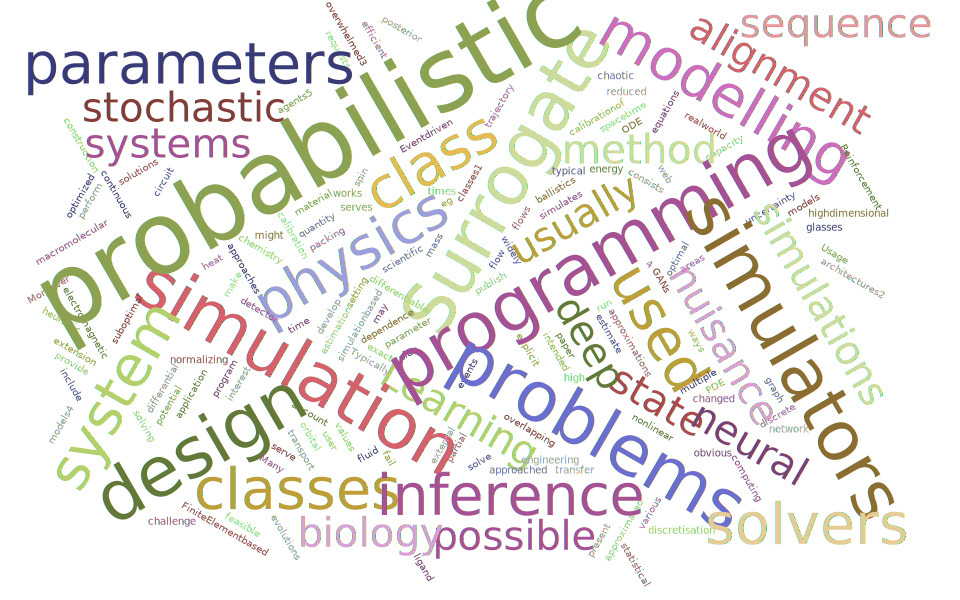
\includegraphics[width=\textwidth]{wordcloud.png}
   \end{figure}
\end{frame}


%%%%%%%%%%%%%%%%%%%%%%%%%%%%%%%%%%%%%%

\begin{frame}
  \frametitle{Demo}
    \textbf{Inverse Simulation}
    \begin{itemize}
      \item <1-> Block coordinates $\sim \mathcal{N}(\mu, \sigma^2)$
      \item <2-> Ball radius $\sim \mathcal{U}(a, b)$
      \item <3-> Ball elasticity $\sim \mathcal{U}(a, b)$
    \end{itemize}
     \begin{figure}
       \href{https://www.youtube.com/watch?v=sVuu3UZmL3w&feature=youtu.be}
          {\includegraphics[height=4cm]{shot1.jpg}}
   \end{figure}
\end{frame}

%%%%%%%%%%%%%%%%%%%%%%%%%%%%%%%%%%%%%%

\begin{frame}
  \centering \Huge
  \emph{Thank You}
\end{frame}

\end{document}
